\chapter{Results}\label{chap:results}
This chapter will present the results achieved in the project as described in Chapter \ref{chap:method}. These results includes comparisons between different models and their hyperparameters but also a look at the different datasets that were used.

\section{Analysis of the datasets}
\label{sec:dataset-summary}
The purpose of this section is to present the result of an investigation into the different datasets. The goal of this was to see if there were any irregularities or patterns in the datasets that could have had an affect on the performance of the networks or the baselines. 
\subsection{5 user data set allvotes}
\label{sec:five-user-data-set}

One thing that we found in the training set for the five user dataset was that the difference in length of the longest title and the second longest title was large. The longest title was 1928 words while the second longest was 66 words. This skewed the variance for the training data and is why one standard deviation sits at $24.9$ as you can see in \ref{table:5-user-set-train} while all the other datasets sits around $10$. If the outlier is removed, one standard deviation is brought down to $9.7$ and sits around the same value as all the other.
\\\\
Another point of interest is how few users share liked titles. In the training set \ref{table:5-user-set-train} you can see that only about $1\%$ of titles have more than 1 up or downvote. In the validation \ref{table:5-user-set-train} and test set \ref{table:5-user-set-train} it is even less titles, $0.45\%$ for the validation and $0.6\%$ for the test set.
\\\\
The data regarding the vote density in subreddits for the $50$ users datasets have been left out simply due to the size of the tables they would require, the data is however available in appendix \ref{appendix:dataset} if the reader is interested.


\begin{table}[H]
    \centering
    \begin{tabular}{ r | c | c | p{4cm}  }
    \hline
    \textbf{User} & \textbf{Active subreddits} & \textbf{Total votes} & \textbf{Votes in two most voted subreddits} \\ \hline \hline
    \multicolumn{4}{c}{\textbf{Training data set}} \\ \hline \hline
    Ayavaron & 64 & 1411 & 444 \\ \hline
    akkartik & 14  & 1387 & 1333 \\ \hline
    crmaki & 14 & 1410 & 902 \\ \hline
    izzycat & 37 & 1363 & 505 \\ \hline
    doctorgonzo & 32 & 1429 & 586 \\ \hline \hline
    \multicolumn{4}{c}{\textbf{Validation data set}} \\ \hline \hline
    Ayavaron & 40 & 416 & 133 \\ \hline
    akkartik & 8  & 392 & 372 \\ \hline
    crmaki & 11 & 390 & 252 \\ \hline
    izzycat & 26 & 428 & 158 \\ \hline
    doctorgonzo & 24 & 364 & 146 \\ \hline \hline
    \multicolumn{4}{c}{\textbf{Testing data set}} \\ \hline \hline
    Ayavaron & 33 & 172 & 60 \\ \hline
    akkartik & 5  & 220 & 212 \\ \hline
    crmaki & 12 & 194 & 131 \\ \hline
    izzycat & 19 & 207 & 77 \\ \hline
    doctorgonzo & 28 & 204 & 78 \\ \hline
    \end{tabular}
    \caption{Vote distribution for the training, validation and testing data sets with five users}
    \label{table:5_user_reddit_dataset}
\end{table}
\todo{Dubbel kolla siffrorna}
\begin{table}[H]
    \centering
    \begin{tabular}{ r | c | c | c }
    \hline
    \textbf{Feature} & \textbf{Training} & \textbf{Validation} & \textbf{Testing} \\ \hline \hline
    \multicolumn{4}{c}{\textbf{Titles}} \\ \hline \hline
    Amount & 6927 & 1983 & 992 \\ \hline
    Median length & 9 & 9 & 8 \\ \hline
    Average length & 12 & 11 & 11  \\ \hline
    Within $\sigma$ title length & 24.9 & 9.6 & 9.4 \\ \hline
    Longer than average & 2198 & 696 & 320 \\ \hline
    More than 1 vote & 76 & 9 & 6 \\ \hline
    More than 2 votes & 2 & 0 & 0\\ \hline \hline
    \multicolumn{4}{c}{\textbf{Subreddits}} \\ \hline \hline
    Amount & 103 & 65 & 59  \\ \hline
    Average voted in in & 32.2 & 21.8 & 19.4 \\ \hline
    Within $\sigma$ voted in & 18.4 & 11.49 & 10.2  \\ \hline
    \end{tabular}
    \caption{Statistics for the dataset containing five users}
    \label{table:5-user-set-train}
\end{table}
\subsection{50 user data set allvotes}
Here there are not any big outliers in title length as in the five user dataset but there is a higher percentage of users that share liked titles compared to the five user dataset. In the training set for the fifty user dataset, $7.75\%$ of titles have more than one up or downvote. In the validation set it is $6\%$ and for the testing set it is $5.7\%$.


\begin{table}[H]
    \centering
    \begin{tabular}{ r | c | c | c }
    \hline
    \textbf{Feature} & \textbf{Training} & \textbf{Validation} & \textbf{Testing} \\ \hline \hline
    \multicolumn{4}{c}{\textbf{Titles}} \\ \hline \hline
    Amount & 63176 & 18486 & 9301 \\ \hline
    Median length & 9 & 9 & 9 \\ \hline
    Average length & 12 & 12 & 12  \\ \hline
    Within $\sigma$ title length & 11.7 & 9.3 & 9.3 \\ \hline
    Longer than average & 23474 & 6736 & 3354 \\ \hline
    More than 1 vote & 5428 & 1231 & 577 \\ \hline
    More than 2 votes & 980 & 220 & 92\\ \hline \hline
    \multicolumn{4}{c}{\textbf{Subreddits}} \\ \hline \hline
    Amount & 343 & 248 & 192  \\ \hline
    Average voted in in & 31.28 & 22.6 & 18.58 \\ \hline
    Within $\sigma$ voted in & 17.6 & 12.17 & 9.88  \\ \hline
    \end{tabular}
    \caption{Statistics for the dataset containing fifty users}
    \label{table:50-user-set-train}
\end{table}

\todo{moar plots/graphs}

As seen in figure \ref{fig:histvotes} most of the posts have a low number of upvotes, this could potentially mean that it is hard to learn from this data.

\begin{figure}[H]
    \centering
    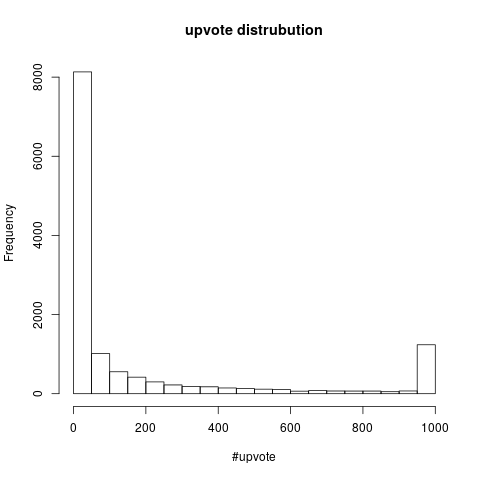
\includegraphics[width=0.75\textwidth]{figure/results/histupvote}
    \caption{A histogram with number of upvote per post on the x axis and number of posts on the y axis.}
    \label{fig:histvotes}
\end{figure}


\section{The first iteration model}
The first iteration of the model was implemented with no hidden layers, as described in section \ref{sec:modelling_the_ann}. It had an LSTM-RNN layer as its input layer with 30 LSTM units. Full details on this model are found in section \ref{sec:app2_first_iter}. When this model was trained on a dataset downscaled to contain five users overfitting was achieved as shown in figure \ref{fig:first_iter_overfitting}.
\begin{figure}[h!]
\begin{subfigure}{0.5\textwidth}
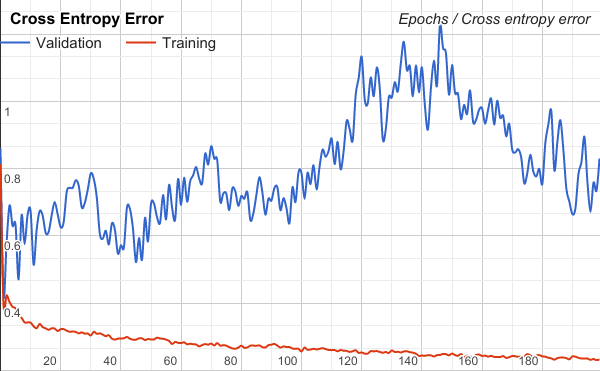
\includegraphics[width=1 \linewidth]{figure/results/first_iter_cross}
\caption{Cross entropy error}
\label{fig:first_iter_overfitting}
\end{subfigure}
\begin{subfigure}{0.5\textwidth}
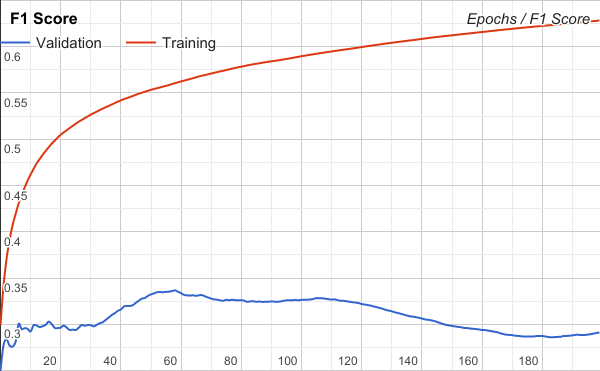
\includegraphics[width=1\linewidth]{figure/results/first_iter_f1}
\caption{$F_1$ score.}
\label{fig:first_iter_f1}
\end{subfigure}
 
\caption{The cross entropy error and $F_1$ score of the first iteration model after 200 training epochs, trained on the training and validation sets. It is good to achieve a low error and a high $F_1$. $F_1$ ranges between $0$ and $1$ inclusive.}
\label{fig:image2}
\end{figure}
\\
The best $F_1$ score achieved on the validation set using the model was $0.3366$, as shown in figure \ref{fig:first_iter_f1}, but the main takeaway was that the model is able to learn from the data.

\section{The final network}
The most optimal network we managed to achieve for the five user dataset had an accuracy of about $39\%$. Even after 1470 epochs this model had not overfitted, however the performance hardly got better after more epochs.

\subsection{Hyperparamaters}
The final result of the hyperparamaters are shown in table \ref{table:hyperparameters_final}

\begin{table}[h!]
    \centering
    \begin{tabular}{ r  p{7cm} }
        \hline
        \textbf{Hyperparamter}  &  \textbf{Value} \\ \hline \hline
        Learning rate & $0.05$  \\ \hline
        Batch Size & $25$ \\ \hline
        RNN units & $400$  \\ \hline
        Embedding Size & t $300$ \\ \hline
        Pre-trained embedding matrix & $False$ \\ \hline
        Trainable embedding matrix & $True$ \\ \hline
        Hidden layers & $1$ \\ \hline
        Neurons in hidden layers & $300$ \\ \hline
        Use L2 regularisation & $True$ \\ \hline
        L2 Factor & $0.01$ \\ \hline
        Dropout regularisation & $True$\\ \hline
        Dropout probability & $0.75$ \\ \hline
        Use constant prediction limit & $False$ \\ \hline
        Constant prediction limit & N/A  \\ \hline
        Use subreddit input & $False$ \\ \hline
    \end{tabular}
    \caption{Final value for all hyperparamaters}
    \label{table:hyperparameters_final}
\end{table}
\section{Baseline comparison} 
\todo{lägga in fina tabeller}
\subsection{Facebook fastText classifier}

\subsection{Random classifier}

\subsection{N-grams}
The F1-score of $0.3898$ was achieved with n-grams when performing on the dataset with five users.
\todo{kör testet med 50 användare sen, GLÖM INTE PLSPLSPLSPLSPLSPLS}

